\begin{annexes}
    \begin{figure}
        \centering
        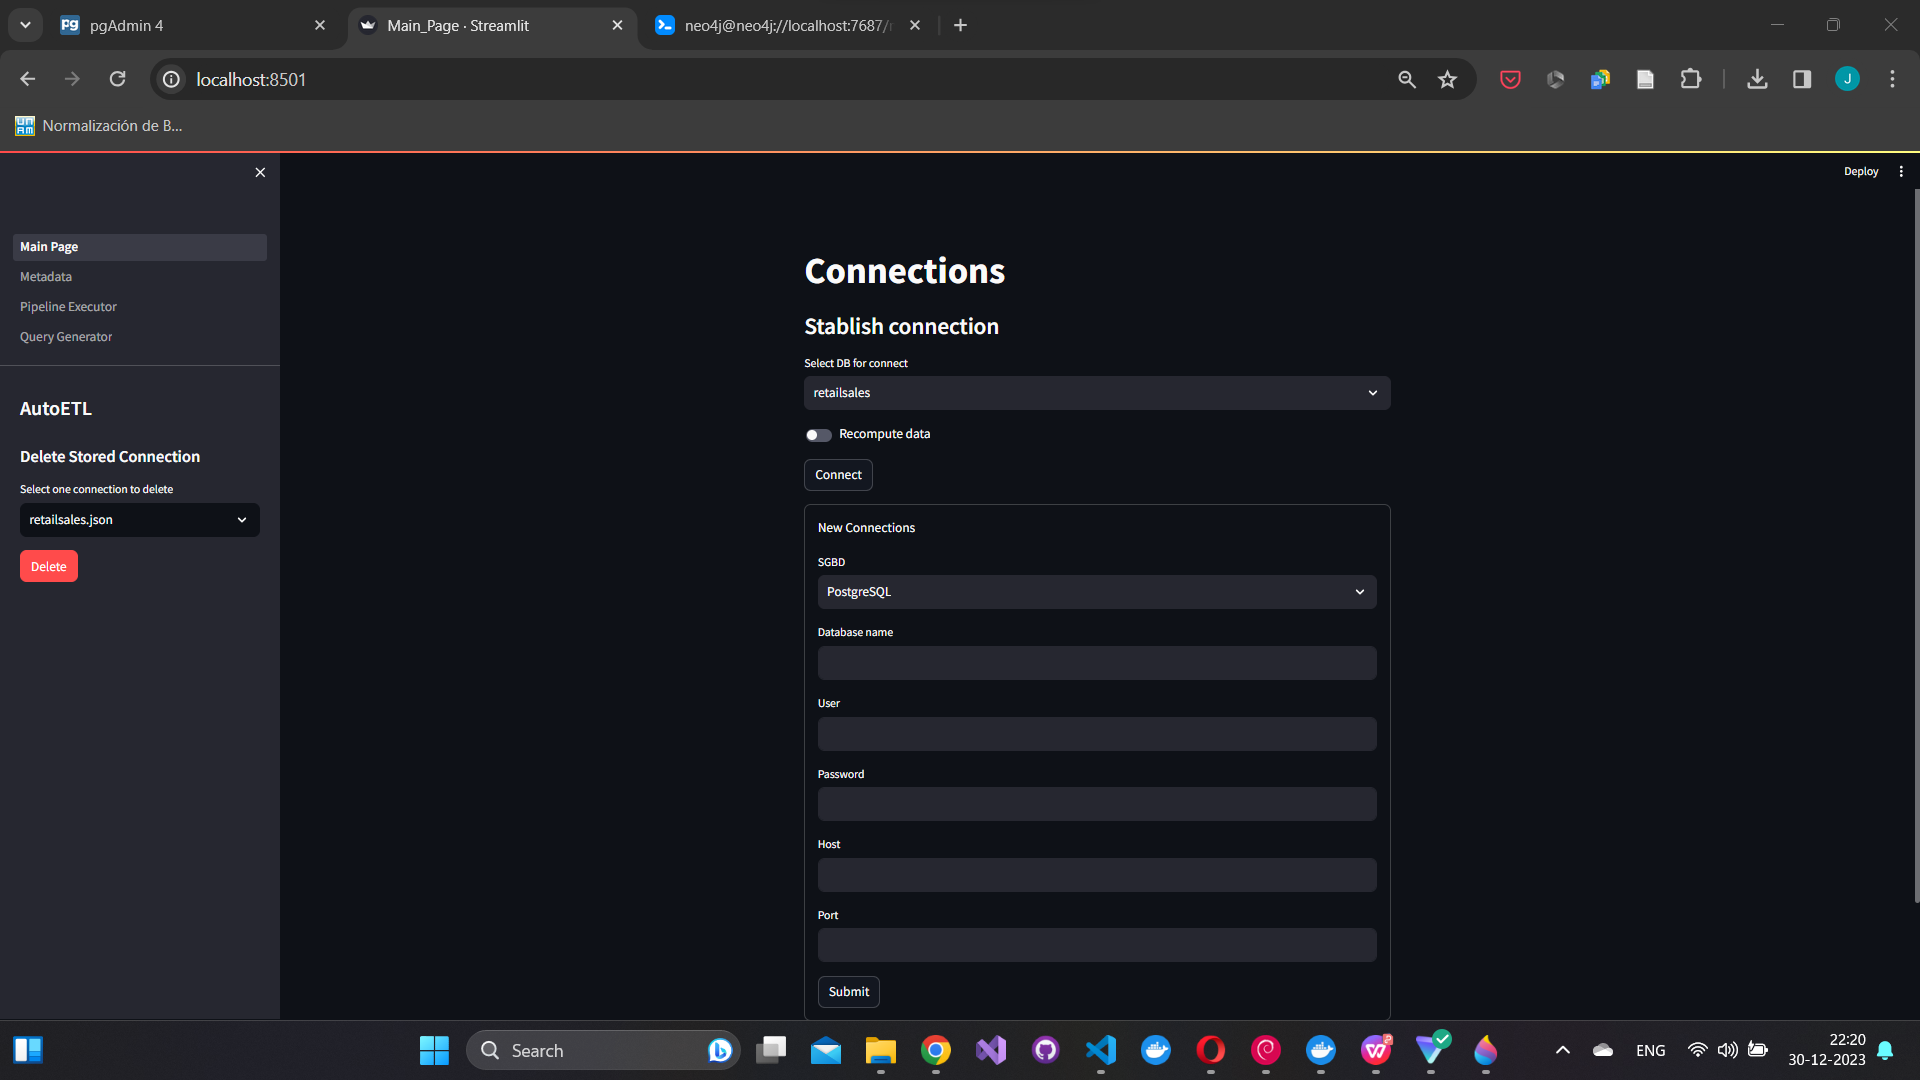
\includegraphics[scale=0.4]{Graphics/mainpage.png}
        \caption{P\'agina principal de la aplicaci\'on.}
        \label{fig:mainpage}
      \end{figure}

    \begin{figure}
        \centering
        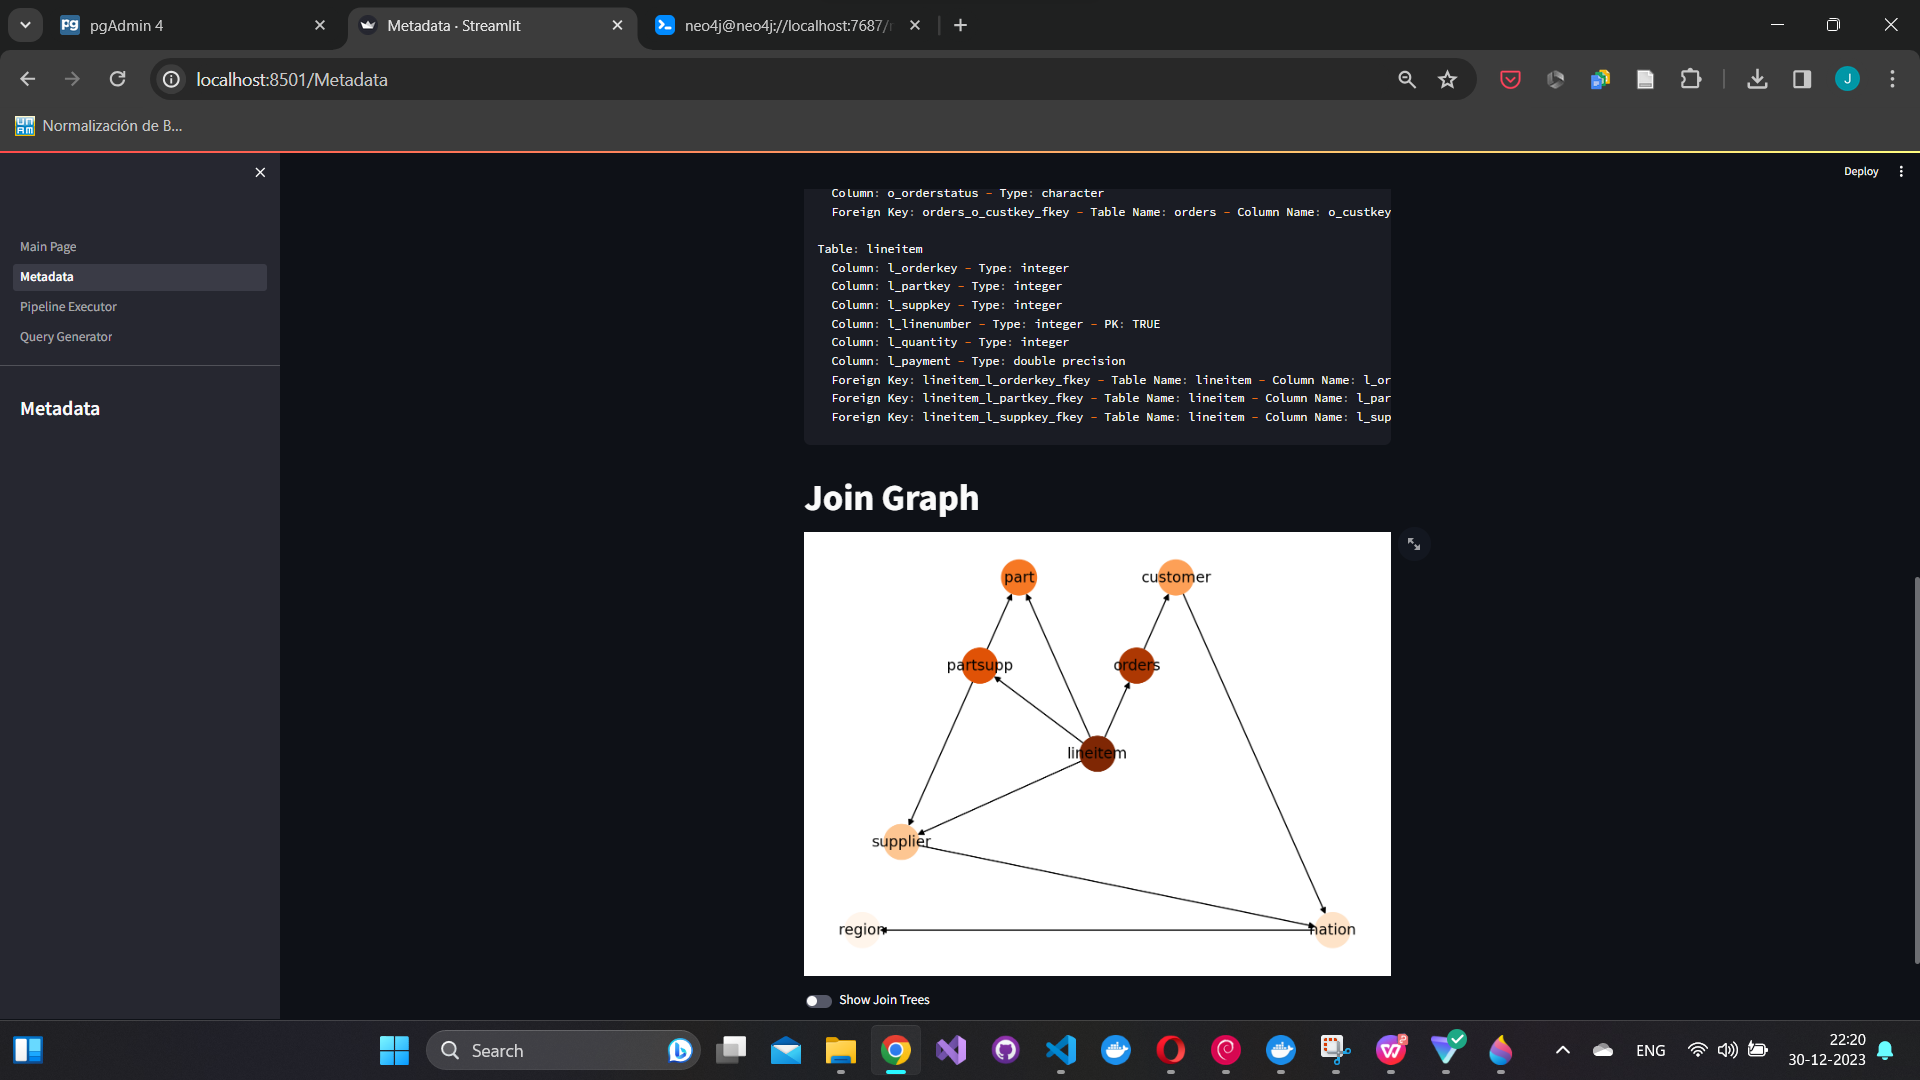
\includegraphics[scale=0.4]{Graphics/metadata.png}
        \caption{P\'agina dedicada a la visualizaci\'on de metadatos de la base de datos fuente conectada.}
        \label{fig:meta}
    \end{figure}

    \begin{figure}
        \centering
        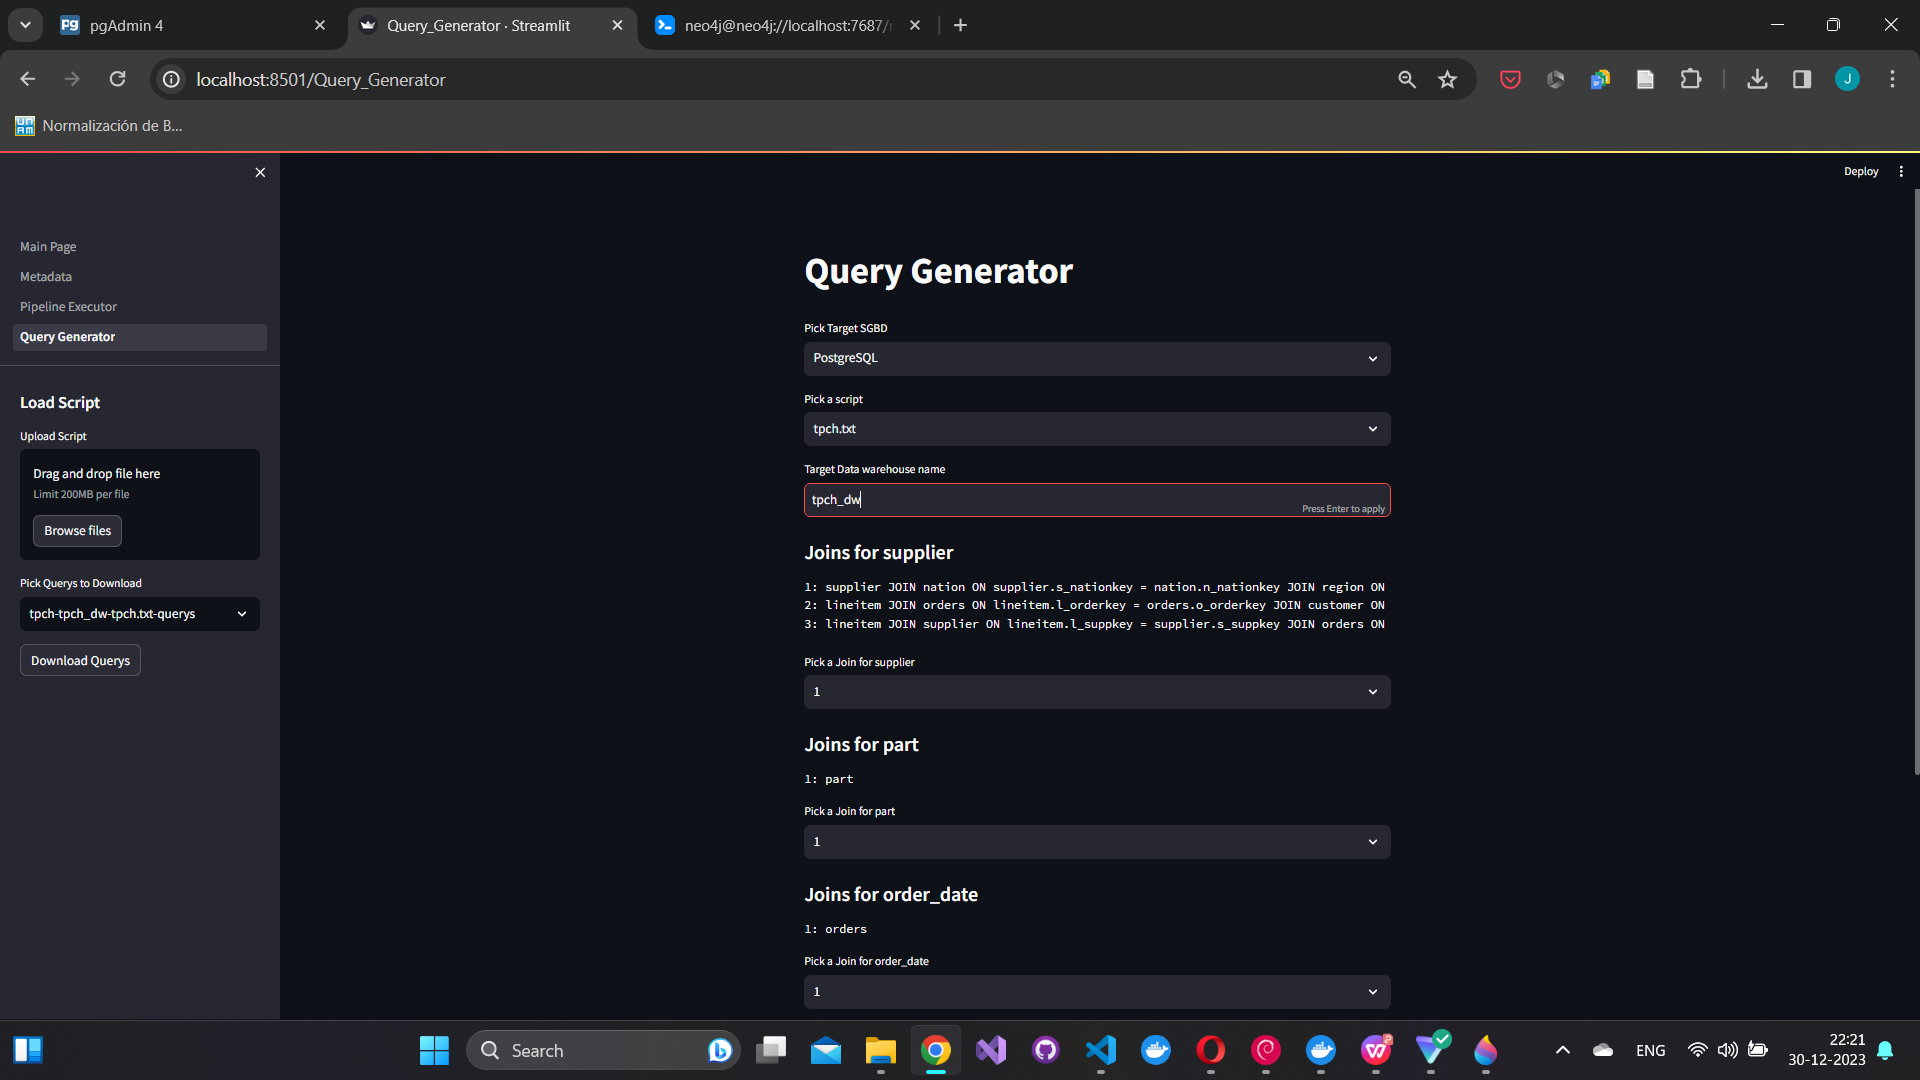
\includegraphics[scale=0.4]{Graphics/querygene.png}
        \caption{P\'agina del generador de consultas.}
        \label{fig:generator}
    \end{figure}

    \begin{figure}
        \centering
        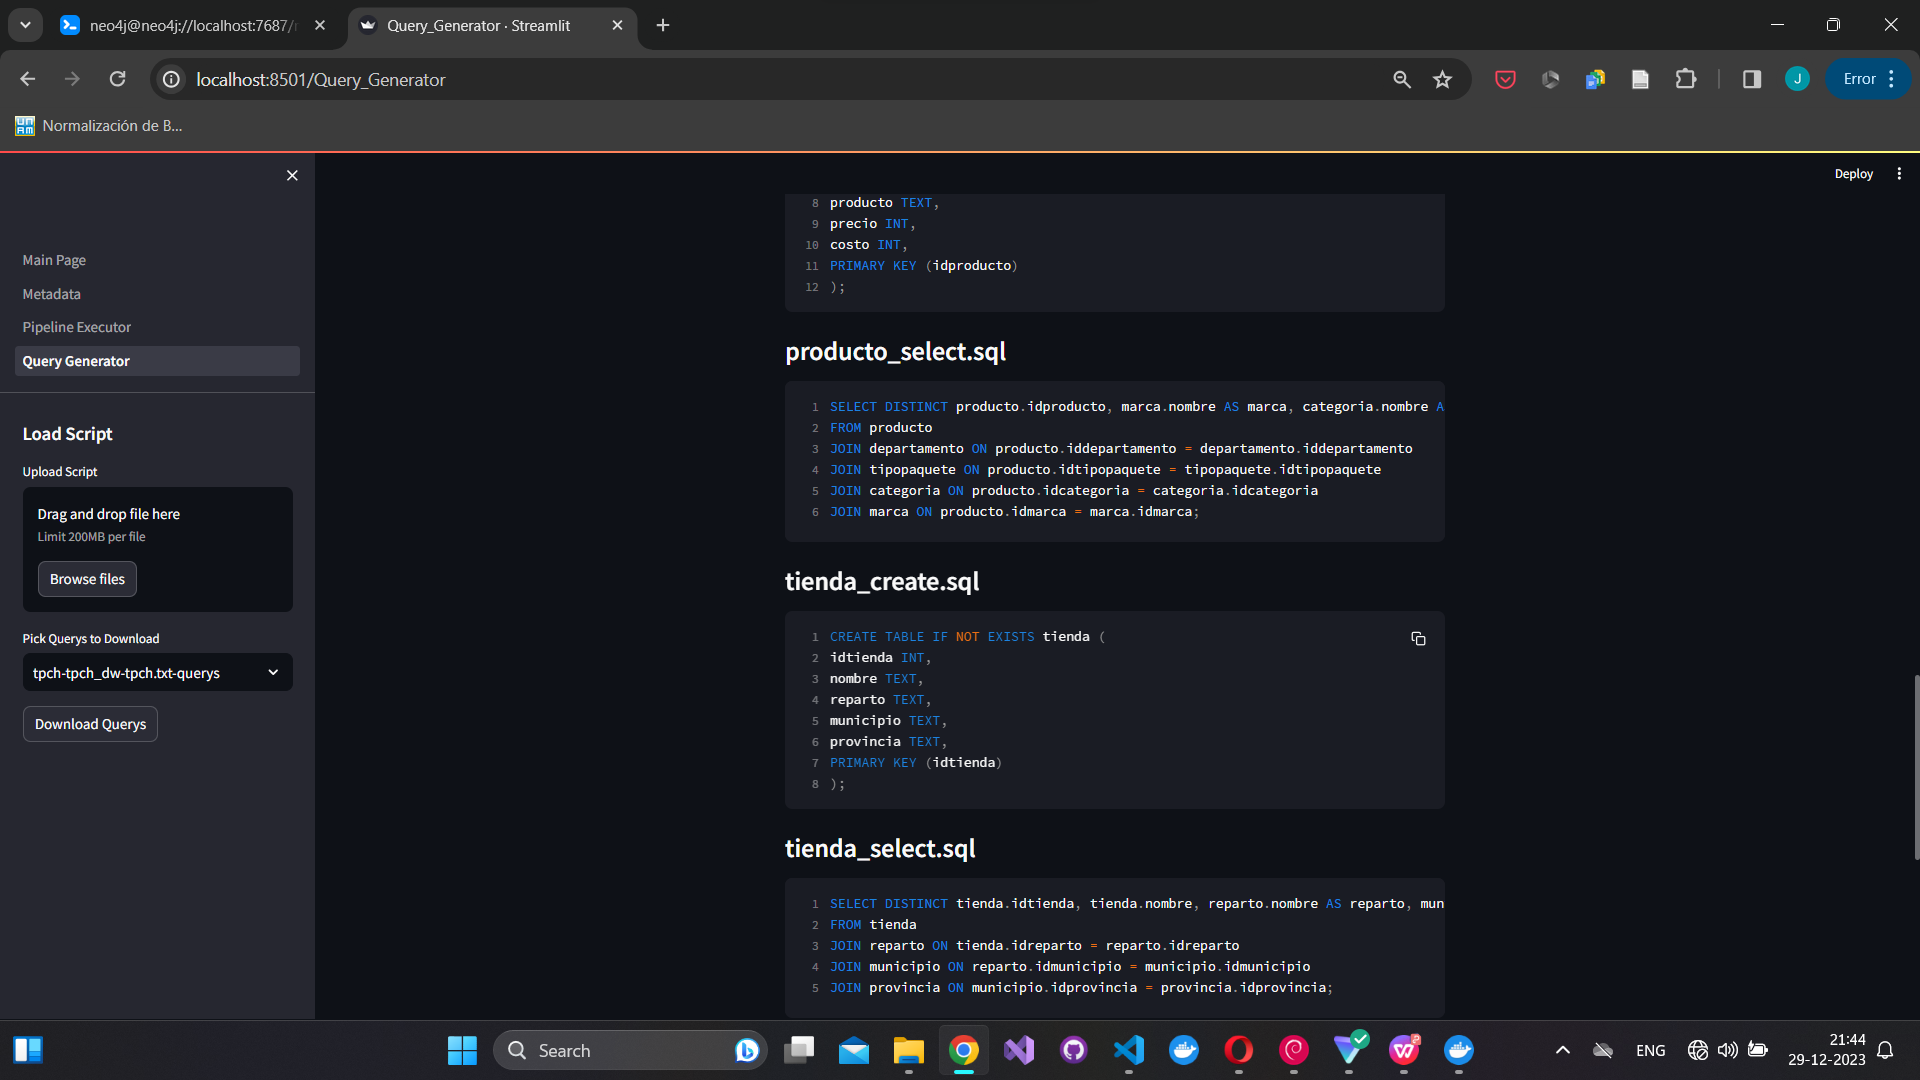
\includegraphics[scale=0.4]{Graphics/generatedquerys1.png}
        \caption{Fragmentos de consultas generadas.}
        \label{fig:qfragment}
    \end{figure}
\end{annexes}